%!tex root=thesis.tex
\chapter{Machine Learning on Crowds}
\label{cha:ml}

In this chapter, we introduce some concepts from machine learning that we will
use for the rest of this thesis. We introduce the classification problem and
some common methods for modelling it, explain how convolutional neural networks
can be used for image feature extraction, discuss the benefits and drawbacks of
crowdsourcing labelling tasks, and introduce some methods to combat label noise
from crowds.

\section{Classification}
\label{sec:classification}

    A common machine learning task, and indeed the machine learning focus of
    this thesis, is \emph{classification}. Given a set $\mathcal X$ of
    \emph{instances} and a set $\mathcal Y$ of \emph{labels}, the classification
    task is to assign a label $y \in \mathcal Y$ to each instance $x \in
    \mathcal X$. The ``true'' label of an instance is called the
    \emph{groundtruth}, and is denoted $z$. Classification thus amounts to
    modelling the conditional distribution $p(z \mid x)$. Some examples of
    classification include labelling images of digits, where $\mathcal X$ is a
    set of images and $\mathcal Y = \{0, \dots, 9\}$ \citep{lecun98}; and
    diagnosing breast cancer in patients, where $\mathcal X$ is a set of sets
    of medical observations and $\mathcal Y$ is the set $\{\text{malignant},
    \text{benign}\}$ \citep{wolberg90}.

    Modelling $p(z \mid x)$ requires some set of \emph{training data} $\mathcal
    D \subset \mathcal X \times \mathcal Y$. The training data are either used
    to find parameters for a model or to estimate the model directly. Both
    processes are called \emph{training} the model. The cardinality of the
    training data is denoted $N = |\mathcal D|$.

    \emph{Binary classification} is classification where each instance must be
    assigned one of two labels, i.e. $\mathcal Y \sim \{0, 1\}$. Instances with
    a true label of $0$ are called \emph{negative instances}, and instances with
    a true label of $1$ are called \emph{positive instances}. For this thesis,
    we will focus entirely on binary classification and set $\mathcal Y = \{0,
    1\}$.

    Instances are usually represented by a vector of \emph{features}, denoted
    $\vec x$. Choosing features is an important and non-trivial part of
    modelling a classification task, and can strongly affect the ability of a
    model to classify instances. The dimensionality of the feature space is
    denoted $D$ and we assume that $\mathcal X \subseteq \mathbb{R}^D$.

    In this section, we look at how to evaluate a classification model, and
    introduce three common ways of modelling binary classification: logistic
    regression, neural networks, and random forests.

    \subsection{Evaluating a Classification Model}
    \label{sec:evaluating-classification-model}

        Given a classification model $y(\vec x)$ that aims to approximate $p(z
        \mid \vec x)$, we want to know how well this model represents the
        groundtruth. In this thesis we make use of two evaluation metrics:
        cross-entropy error, and balanced accuracy.

        The \emph{cross-entropy error} \citep{bishop06} is a common method for
        evaluating a binary classification model. The cross-entropy error is
        given by
        \[
            L(\mathcal D) = -\frac{1}{N} \sum_{\vec x, z \in \mathcal D} \left(
                z \log y(\vec x) + (1 - z) \log (1 - y(\vec x))
            \right).
        \]
        Higher error indicates a ``worse'' model.

        The \emph{balanced accuracy} is another common method of evaluating
        classification models. It is the average of the accuracy of classifying
        positive instances and the accuracy of classifying negative instances,
        i.e.
        \[
            a = \frac{1}{2} \left(\frac{p_{\text{true}}}{p} + \frac{n_{\text{true}}}{n}\right),
        \]
        where $p$ is the number of instances with $z = 1$, $n$ is the number of
        instances with $z = 0$, $p_{\text{true}}$ is the number of correctly
        classified instances with $z = 1$, and $n_{\text{true}}$ is the number
        of correctly classified instances with $z = 0$.

        Unless otherwise specified, we use the cross-entropy error for training
        our models, and report the balanced accuracy.

    \subsection{Logistic Regression}
    \label{sec:logistic-regression}

        Logistic regression is a simple linear model of binary classification
        \citep{bishop06}. The conditional distribution $p(z \mid \vec x)$ is
        modelled as
        \begin{equation}
            \label{eq:logistic-regression}
            y(\vec x) = p(z = 1 \mid \vec x) = \sigma(\vec w^T \vec x + b),
        \end{equation}
        where $\vec w$ and $b$ are parameters to the model and $\sigma$ is the
        logistic sigmoid function
        \[
            \sigma(t) = \frac{1}{1 + \exp(-t)}.
        \]
        The elements of $\vec w$ are called the \emph{weights}, and control the
        effect of each feature on the output label probability. $b$ is the
        \emph{bias}, a constant added to all weighted sums of features
        independent of the features themselves. $b$ can be incorporated into
        $\vec w$ by adding an extra feature to $\vec x$ that is always $1$ and
        increasing the dimension of $\vec w$ by 1. I adopt this convention for
        the remainder of this thesis whenever $b$ is not explicitly included.

        Logistic regression is differentiable, and so may be trained using
        \emph{gradient descent}. In gradient descent, $\vec w$ is modified by
        the update equation
        \[
            \vec w \leftarrow \vec w - \lambda \nabla L(\vec w),
        \]
        where $L : \mathbb{R}^D \to \mathbb{R}$ is the \emph{loss} function and
        $\lambda \in (0, 1)$ is the \emph{learning rate}.

        The loss function represents how well the current model fits the
        observations. For binary classification, this is usually given by the
        cross-entropy error with gradient \citep{bishop06}
        \[
            \nabla L(\vec w) = -\frac{1}{N}
                \sum_{\vec x, z \in \mathcal D} \left(z - y(\vec x)\right) \vec x.
        \]

    \subsection{Neural Networks}
    \label{sec:neural-networks}

        One key limitation of logistic regression is that it is a linear model.
        This means that the decision boundary is a hyperplane in the feature
        space, and thus logistic regression can only classify data with classes
        that are linearly separable. In general, classes may not be linearly
        separable, so logistic regression may not be able to accurately model
        the classification task. One way to improve logistic regression
        performance on non-linearly separable classes is to introduce a
        nonlinear \emph{feature map} $\vec\phi : \mathbb{R}^D \to \mathbb{R}^F$
        to transform the inputs. Logistic regression then becomes
        \[
            y(\vec x) = \sigma(\vec w^T \vec\phi(\vec x)).
        \]
        By judicious choice of feature transformations, the features may be
        transformed into a space where the classes are linearly separable. This
        raises a question: What feature map should we choose?

        We can approximate the feature map by a simple linear function, i.e.
        \[
            \vec\phi(\vec x) = \vec\sigma(A \vec x),
        \]
        where $\vec\sigma(\vec v)$ is $\sigma$ applied elementwise to $\vec v$.
        The weight matrix $A$ can then be learned by gradient methods along with
        $\vec w$. This approximation itself has drawbacks --- perhaps a linear
        function is not powerful enough to approximate a good choice of feature
        map --- but we can resolve this by applying another nonlinear
        transformation to $\vec x$, arbitrarily many times. This leads to a new
        model with multiple weights $A_1, \dots, A_k$:
        \begin{align*}
            y(\vec x) &= \sigma(\vec w^T \vec\phi_1(\vec x))\\
            \vec\phi_1(\vec x) &= \vec\sigma(A_1 \vec\phi_2(\vec x))\\
            &\vdots\\
            \vec\phi_K(\vec x) &= \vec\sigma(A_K \vec x).
        \end{align*}
        This is a \emph{$K$-layer neural network}, so called as it resembles
        the structure of neurons in the brain. Such a network is able to
        approximate any function with sufficiently large dimensionality of the
        matrices $A_i$ \citep{gybenko89}.

        While we have viewed neural networks here as a very natural extension
        to logistic regression, the class of neural network models is far more
        varied. Interpreting each element in $\vec x, \vec \phi_K, \dots, \vec
        \phi_1$ as a node and the elements of $A_K, \dots, A_1, \vec w$ as
        weighted edges, we can interpret the above neural network as a directed
        acyclic graph (Figure \ref{fig:nn-as-dag}). In this context, each column
        of the graph is called a \emph{layer}. If the layer is fully connected
        to its inputs and outputs, then it is called a \emph{dense layer}. We
        may also introduce different kinds of layers performing arbitrary
        nonlinear functions; some examples of these will be covered in Section
        \ref{sec:convolutional-neural-networks}.

        \begin{figure}
            \centering
            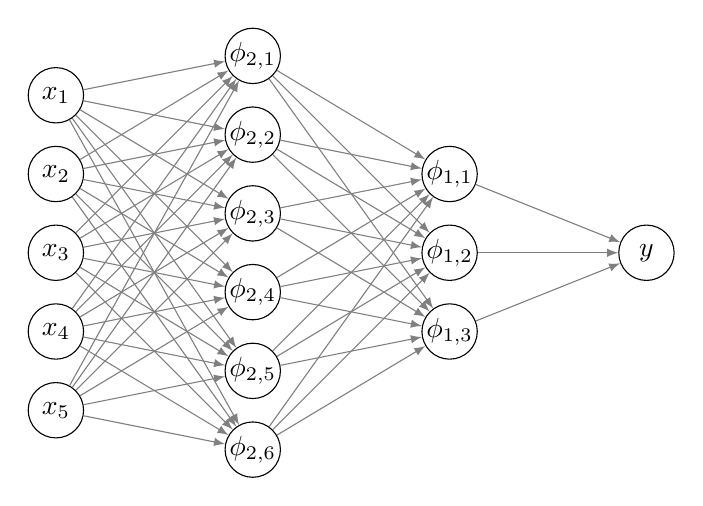
\begin{tikzpicture}[scale=0.5, node distance=2.5cm]
                \tikzstyle{neuron}=[
                    circle, draw, minimum size=20pt, inner sep=0pt]
                \tikzstyle{connector}=[->, arrows={-latex}, black!50]
                \foreach \name / \y in {1, ..., 5}
                    \node [neuron] (I-\name) at (0, -\y*2) {$x_\y$};

                \foreach \name / \y in {1, ..., 6}
                    \node [neuron] (P1-\name)
                        at (5, -\y*2 + 1) {$\phi_{2, \y}$};

                \foreach \name / \y in {1, ..., 3}
                    \node [neuron] (P2-\name)
                        at (10, -\y*2 - 2) {$\phi_{1, \y}$};

                \node [neuron] (y) at (15, -6) {$y$};

                \foreach \source in {1, ..., 5}
                    \foreach \dest in {1, ..., 6}
                        \path [connector] (I-\source) edge (P1-\dest);

                \foreach \source in {1, ..., 6}
                    \foreach \dest in {1, ..., 3}
                        \path [connector] (P1-\source) edge (P2-\dest);

                \foreach \source in {1, ..., 3}
                    \path [connector] (P2-\source) edge (y);
            \end{tikzpicture}
            \caption{A 2-layer neural network represented as a directed acyclic
                graph.}
            \label{fig:nn-as-dag}
        \end{figure}

    \subsection{Random Forests}
    \label{sec:random-forests}

        \begin{itemize}
            \item Random forests are a classification method using an ensemble of decision trees
            \item Decision trees are generated with access to only a subset of features or instances
            \item Each decision tree votes for a classification
            \item Majority vote
            \item cite http://math.bu.edu/people/mkon/MA751/L18RandomForests.pdf
        \end{itemize}

\section{Feature Extraction from Images}
\label{sec:image-feature-extraction}
    
    For instances to be input to a classification model, they must be
    represented by vectors of features. Feature selection is generally a hard
    problem, but it may be straightforward if instances are simple vectors of
    measurements (such as in the breast cancer dataset described in Section
    \ref{sec:breast-dataset}). If the instances are provided in the form of
    images, however, feature selection becomes considerably harder.

    \subsection{The Na\"ive Approach}
    \label{sec:naive-approach-image-features}

        Images can be thought of as vectors of pixels, where the value of each
        pixel is treated as an independent feature. If the image is a colour
        image, then each channel (red, blue, and green) of each pixel can be
        treated as an independent feature. This is a very simple way to obtain
        features from images, with two considerable problems.

        \begin{figure}
            \centering
            \begin{subfigure}[t]{0.5\textwidth}
                \centering
                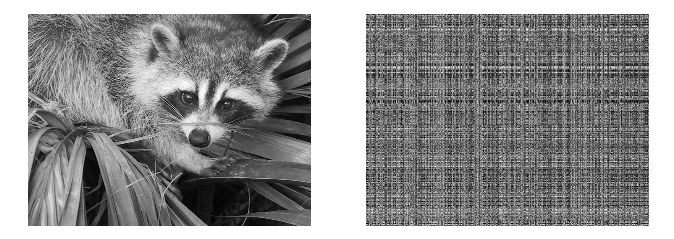
\includegraphics[width=\textwidth]{images/face.png}
            \end{subfigure}%
            ~
            \begin{subfigure}[t]{0.5\textwidth}
                \centering
                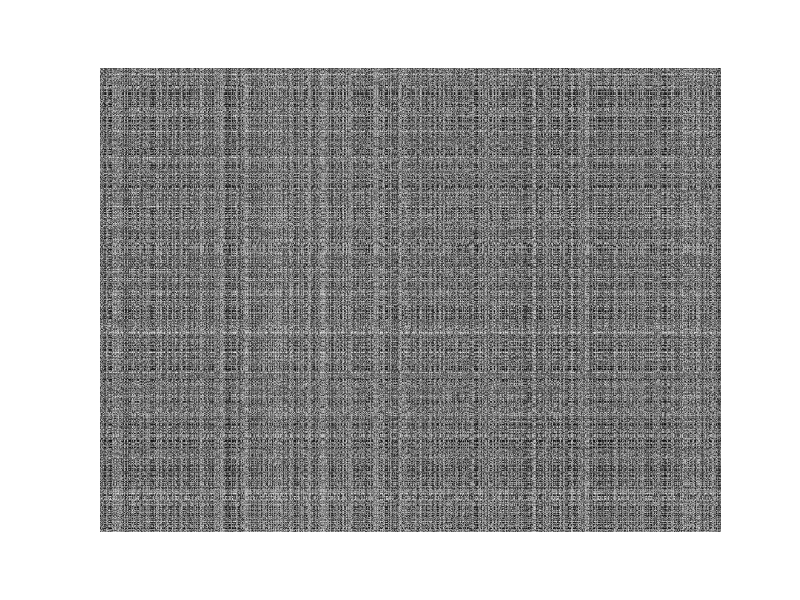
\includegraphics[width=\textwidth]{images/face_shuffled.png}
            \end{subfigure}
            \caption{If we ignore the location of pixels when interpreting an
                image as a vector, these two images have identical feature
                vectors, despite the left image clearly containing information
                not present in the right image.}
            \label{fig:shuffled-face}
        \end{figure}

        The first problem is that using pixels directly as independent features
        fails to accurately capture the image. The pixels are assumed
        independent when this is not the case --- neighbouring pixels are likely
        to be correlated, shapes and structure within the image introduce
        further correlations, and so on. If we are only looking at certain kinds
        of images, then the pixel location may also matter --- for example, we
        might have as inputs photographs of landscapes, where the sky tends to
        be at the top of the image --- and this information is also lost. These
        effects are shown in Figure \ref{fig:shuffled-face}. Finally, with
        independent pixels as features, trained models will be sensitive to
        small distortions or translations in the input \citep{lecun98}. In
        Section \ref{sec:convolutions}, we describe a common approach for
        resolving this problem.

        The second problem with this approach is that images tend to be large
        \citep{lecun98}. Taking each pixel as a feature leads to high
        dimensional feature spaces. This is not ideal as many algorithms perform
        poorly in high dimensional spaces. This can be resolved using
        \emph{pooling}, which we describe in Section \ref{sec:pooling}.

    \subsection{Pooling}
    \label{sec:pooling}

        \begin{figure}
            \centering
            \begin{subfigure}[t]{0.5\textwidth}
                \centering
                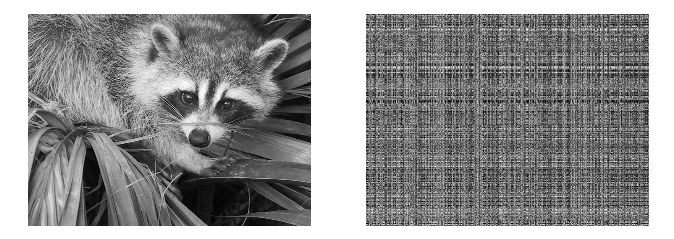
\includegraphics[width=\textwidth]{images/face.png}
                \caption{Original image.}
                \label{fig:pooling-face-original}
            \end{subfigure}%
            ~
            \begin{subfigure}[t]{0.5\textwidth}
                \centering
                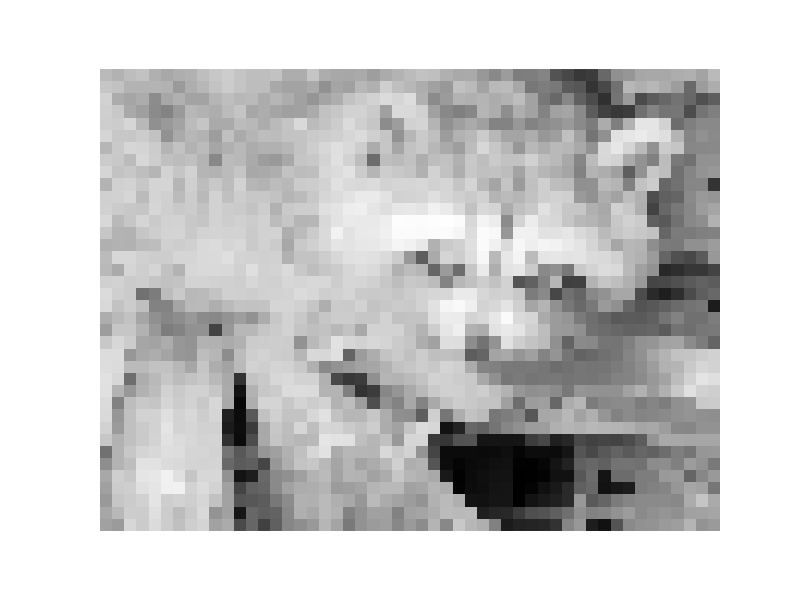
\includegraphics[width=\textwidth]{images/face_max_pooled.png}
                \caption{Max pooling.}
                \label{fig:pooling-face-max}
            \end{subfigure}
            \begin{subfigure}[t]{0.5\textwidth}
                \centering
                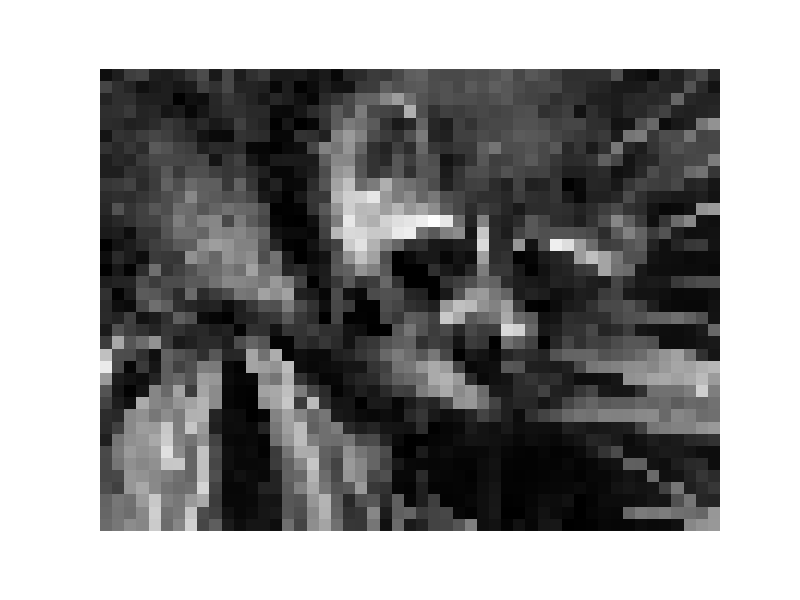
\includegraphics[width=\textwidth]{images/face_min_pooled.png}
                \caption{Min pooling.}
                \label{fig:pooling-face-min}
            \end{subfigure}%
            ~
            \begin{subfigure}[t]{0.5\textwidth}
                \centering
                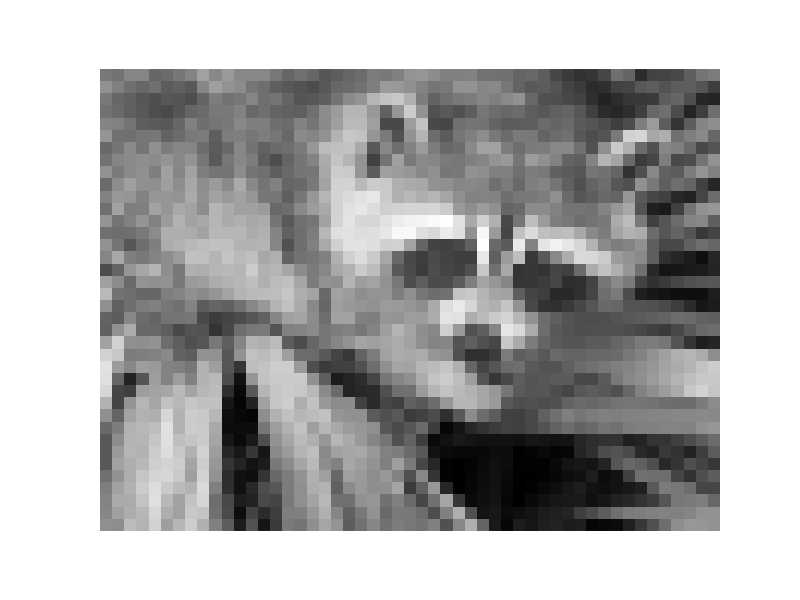
\includegraphics[width=\textwidth]
                    {images/face_average_pooled.png}
                \caption{Average pooling.}
                \label{fig:pooling-face-average}
            \end{subfigure}%
            \caption{Examples of max, min, and average pooling applied to an
                image.}
            \label{fig:pooling}
        \end{figure}

        Pooling is a class of operations that reduce the dimensionality of an
        image, parameterised by a \emph{pool size}\footnote{Another
        parameter is the \emph{stride}, $s$, which we ignore here for simplicity,
        setting $s = p$.}, $p$. Nonoverlapping $p \times p$ squares of pixels are
        condensed into one value, which becomes the corresponding pixel in the
        output. In this way, the size of the image is reduced from $m \times n$
        to $\frac{m}{p} \times \frac{n}{p}$. This results in both a smaller
        amount of data, and some amount of translation invariance when pooling
        is used in models like neural networks \citep{scherer10}.

        We are free to choose whatever aggregation operation we like to condense
        squares of pixels; common choices are $\max$ (called \emph{max pooling})
        and $\mbox{mean}$ (called \emph{average pooling}). Some pooling examples
        are shown in Figure \ref{fig:pooling}.

    \subsection{Convolutions}
    \label{sec:convolutions}

        \begin{figure}
            \centering
            \begin{subfigure}[t]{0.3\textwidth}
                \centering
                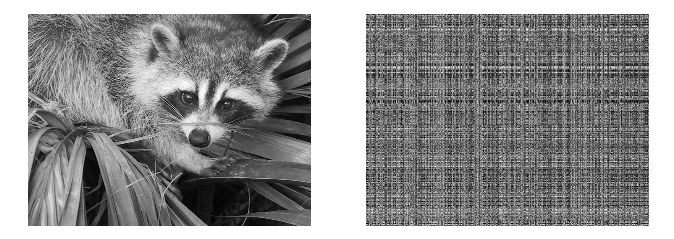
\includegraphics[width=\textwidth]{images/face.png}
                \caption{Original image.}
                \label{fig:convolution-face-original}
            \end{subfigure}%
            ~
            \begin{subfigure}[t]{0.3\textwidth}
                \centering
                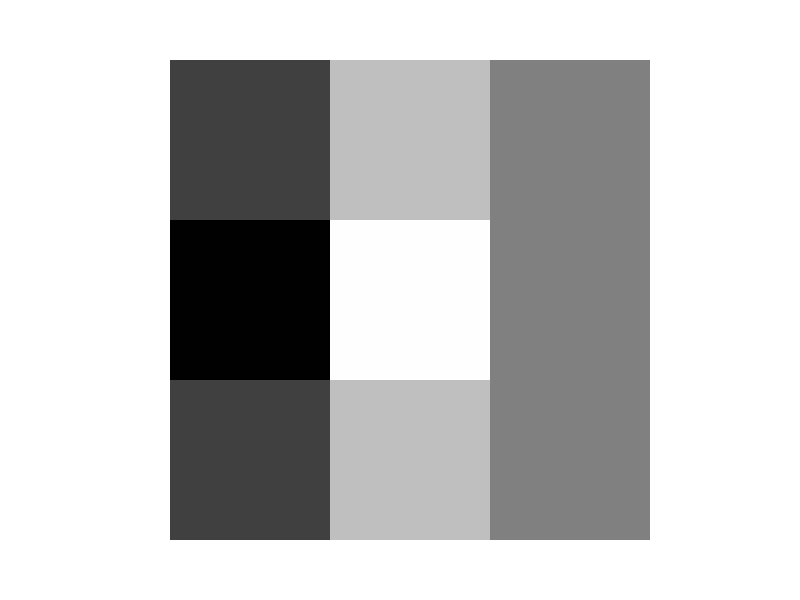
\includegraphics[width=\textwidth]
                    {images/convolutional_filter.png}
                \caption{Convolutional filter.}
                \label{fig:convolution-face-filter}
            \end{subfigure}%
            ~
            \begin{subfigure}[t]{0.3\textwidth}
                \centering
                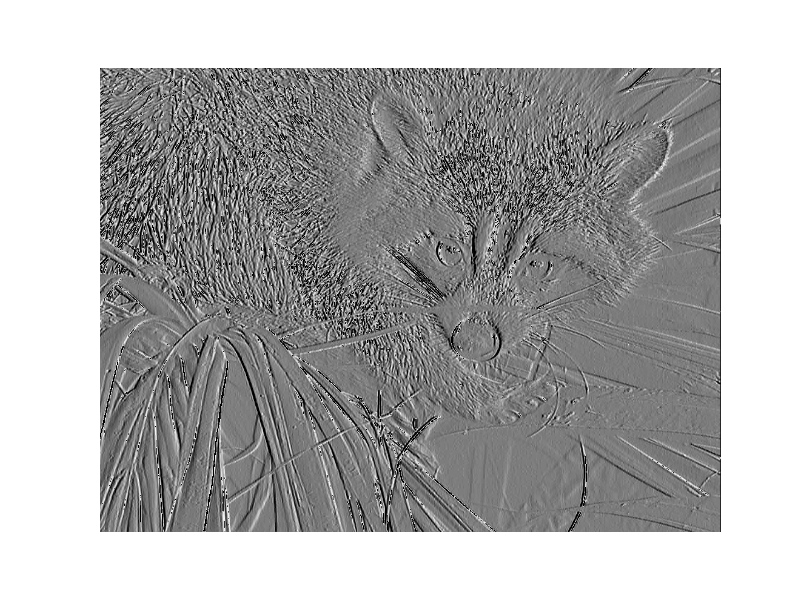
\includegraphics[width=\textwidth]{images/face_convolved.png}
                \caption{Convolved image.}
                \label{fig:convolution-face-convolved}
            \end{subfigure}
            \caption{Convolving an image with a $3 \times 3$ filter gives a new
                image. This filter acts as a kind of vertical edge detector.}
            \label{fig:convolved-face}
        \end{figure}

        A common way to make use of neighbourhood information in images is by
        using \emph{convolutions}. A convolution is an operation that transforms
        an image by applying an $n \times n$ \emph{filter} to each $n \times n$
        square of pixels. The filter is a matrix in $\mathbb{C}^{n \times n}$,
        and it is applied to a square of pixels by treating that square as a
        matrix, performing an elementwise multiplication between the filter
        matrix and the pixel matrix, and summing the result. Applying the filter
        to a square of pixels gives a single pixel value, so by applying the
        filter across the image, a new image is generated \citep{ludwig15}.

        One ambiguity is how to apply a filter to the edges of an image. There
        are multiple ways to resolve this. The most common method is to only
        apply the filter to squares of pixels fully contained within the image,
        making the output image smaller than the input. Another method is to
        apply the filter to the edges and assume that pixels outside the image
        have a constant value (usually 0), making the output image the same size
        as the input. These methods are commonly known as ``valid'' and ``same''
        respectively in libraries such as SciPy and Keras.

        The effect of a simple convolutional filter on an image is shown in
        Figure \ref{fig:convolved-face}, and an algorithm for performing a
        convolution is shown in Algorithm \ref{alg:convolution}.

        \begin{algorithm}
            \KwData{\\\quad{}An image $X \in \mathbb{R}^{m \times n}$%
                    \\\quad{}A filter $F \in \mathbb{C}^{d \times d}$}
            \KwResult{An image $\in
                \mathbb{R}^{(m - d + d \text{ mod } 2) \times
                            (n - d + d \text{ mod } 2)}$}

            Initialise output image $Y \in \mathbb{R}^{(m - d + d \text{ mod } 2) \times (n - d + d \text{ mod } 2)}$\;
            \For{$y \in \lfloor d/2 \rfloor, \dots, m - \lfloor d/2 \rfloor$}{
                \For{$x \in \lfloor d/2 \rfloor, \dots, n - \lfloor d/2 \rfloor$}{
                    $H \leftarrow$ $d \times d$ square of pixels centred on $(x, y)$\;
                    $Y_{y, x} \leftarrow (\vec 1^T (H \odot F) \vec 1) / (\vec 1^T F \vec 1)$\;
                }
            }

            \KwRet{$Y$}
            \caption{One method of performing a convolution. Here, we choose to
                use the ``valid'' method of handling edges, resulting in a
                smaller output than the input. $\odot$ is the elementwise
                matrix product.}
            \label{alg:convolution}
        \end{algorithm}

        By repeatedly applying convolutions and pooling, we can extract features
        from images that would not have been present using the na\"ive approach
        of Section \ref{sec:naive-approach-image-features}.

        \begin{itemize}
            \item CNNs are widely used now that we have a lot of data
            \item Robust and require minimal pre-processing (cite 21)
        \end{itemize}

    \subsection{Convolutional Neural Networks}
    \label{sec:convolutional-neural-networks}

        \begin{figure}
            \centering
            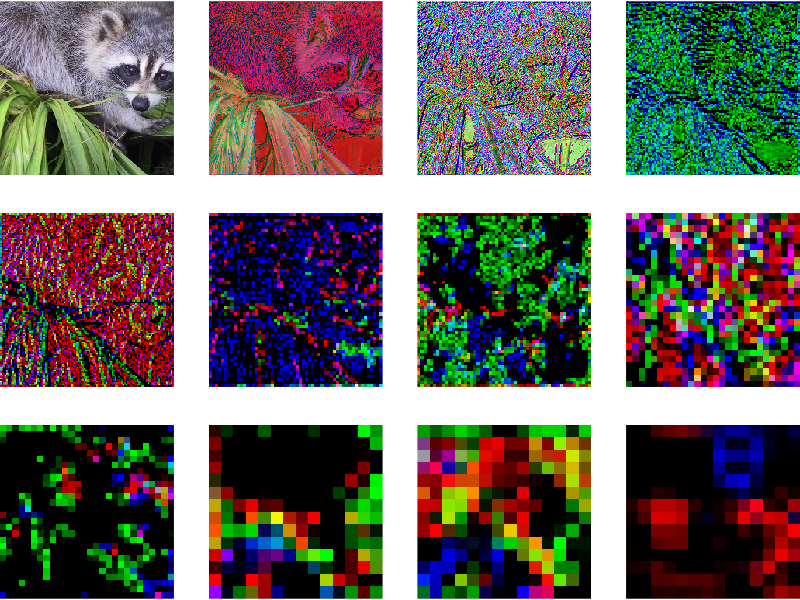
\includegraphics[width=\textwidth]{images/face_cnn.png}
            \caption{A convolutional neural network applied to the top-left
                image. The other images are the outputs of intermediate
                convolutional layers of the neural network, from left to right,
                top to bottom. Colours represent convolutions with different
                filters. The output, bottom-right, is a higher-level
                representation of the input image, and its values can be used
                as inputs for classification. This figure uses
                \citeauthor{baraldi15}'s implementation of the VGG-16 CNN
                \citep{simoyan14}.}
            \label{fig:face-cnn}
        \end{figure}

        While convolutions are needed to extract features from our images, there
        are no convolutions that work well in general. Convolutions must be
        chosen on a domain-dependent basis. This raises the question: What
        convolutions should we choose?

        One way to answer this question is simply to not choose at all, and
        then learn the appropriate convolutions as part of a larger
        classification model. This gives rise to the concept of a
        \emph{convolutional neural network} (CNN). A CNN is a neural network
        with layers that convolve their inputs and layers that pool their
        inputs, called \emph{convolutional layers} and \emph{pooling layers},
        respectively. Convolutional layers may contain any number of separate
        filters. They are generally interspersed with pooling layers. The final
        layers of the CNN are usually dense layers. Additionally, CNNs introduce
        some amount of translation invariance into their outputs, since the same
        filters are applied across the image \citep{lecun98}.

        CNNs can be used for feature extraction from images. As input, they
        take images to extract features from, and they are tasked with mapping
        these to some meaningful value or the intended output of the greater
        classification problem. The convolutional and pooling layers can then
        be isolated, forming a network that extracts features from images. An
        example of a convolutional neural network applied to an image is shown
        in Figure \ref{fig:face-cnn}.

\section{Crowdsourcing Labels}
\label{sec:crowdsourcing}

    For standard supervised learning tasks, the labels are generally provided by
    some \emph{expert}. We assume that the expert provides labels that are
    correct and accurately represent the groundtruth. More recently, however,
    many projects have \emph{crowdsourced} their labels: Non-expert people (the
    \emph{crowd}) volunteer or are paid to label data. The crowd may be sourced
    from websites like Amazon Mechanical Turk\footnote{\url{http://mturk.com}}
    where small amounts of money are paid on a per-label basis, or they may
    volunteer out of interest in the labelling project.

    Crowdsourcing allows us to quickly and cheaply label large amounts of data.
    This comes at the expense of objectivity and reliability --- since the crowd
    are necessarily non-experts, they do not have domain knowledge for the
    problem, and may not provide high-quality labels \citep{raykar10}. While we
    can try to reduce noise by requesting multiple labellers label each instance
    \citep{lin16, sheng08}, this does not address the fact that the data may be
    intrinsically hard to label, the labellers may be correlated, and some
    labellers may even be actively malicious \citep{yan10}. Some strategies to
    address these problems are described in Section \ref{sec:crowd-labels}.

    % The most obvious advantage of crowdsourcing is that crowds are able to
    % cheaply or quickly label large amounts of data simply because there are so
    % many people labelling. Crowds also allow us to gather labels on a wide
    % range of data

    The form of crowdsourcing we are interested in for this thesis is
    \emph{citizen science}, as this is form of crowdsourcing that the Radio
    Galaxy Zoo (Section \ref{sec:radio-galaxy-zoo}) uses. Citizen science is
    ``scientific work undertaken by members of the general public''
    \citep{oed-citizenscience, marshall15}, and has recently come to refer
    mainly to websites that allow non-experts to label scientific data. A
    notable example of citizen science is the Galaxy Zoo project
    \citep{lintott08}, which aims to identify morpologies of galaxies from the
    Sloan Digital Sky Survey. Galaxy Zoo has gathered tens of millions of labels
    for nearly $9 \times 10^5$ galaxies from over $8 \times 10^4$ volunteers
    \citep{lintott11}, and the data collected have been used in 48 publications
    so far\footnote{\url{https://www.zooniverse.org/about/publications}}. Many
    other citizen science projects have been hosted on the Galaxy Zoo's
    platform, Zooniverse\footnote{\url{http://zooniverse.org}}, from further
    astronomical studies like the Radio Galaxy Zoo \citep{banfield15} (Section
    \ref{sec:radio-galaxy-zoo}), which itself has labelled over $10^5$ radio
    sources from two radio surveys; to ecological studies like Snapshot
    Serengeti \citep{swanson15}, which has classified nearly 11 million camera
    trap images from Serengeti National Park.

    % Crowdsourcing is not without downsides. Since the crowd necessarily
    % consists of non-experts, there is no longer any guarantee that labels are
    % correct --- indeed, for the Radio Galaxy Zoo, balanced accuracy of
    % individual labellers varies from 40--100\%, with an average of 71\%.
    % Additionally, labels from different labellers may be correlated, different
    % labellers may be better skilled at labelling different kinds of examples,
    % some examples may be intrinsically hard for non-experts to label, and
    % labellers may even be actively malicious in giving incorrect labels
    % \citep{yan11}.

\section{Simulating a Crowd Labelling Task}
\label{sec:crowd-simulation}

    The crowd is inherently unpredictable. This makes it difficult to test
    methods for crowd learning, since there may be biases in existing
    crowd-labelled datasets, and we want our experiments to be both accurate and
    reproducible. To mitigate this problem, we instead simulate a crowd
    labelling task based on a dataset with known groundtruth. In this section,
    we describe our method for simulating a crowd labelling task, which we will
    later employ to test methods in Section \ref{sec:crowd-labels}. As part of
    this thesis, we have also implemented this simulation in Python. The
    implemention is described in Section \ref{sec:crowdastro-util}.

    \subsection{The Breast Cancer Wisconsin Dataset}
    \label{sec:breast-dataset}

        The breast cancer Wisconsin dataset, first used by
        \citeauthor{wolberg90}, presents a classification task commonly used for
        testing classification methods. The dataset can be obtained from the UCI
        Machine Learning Repository \citep{lichman13}
        \footnote{\url{https://archive.ics.uci.edu/ml/%
                       datasets/Breast+Cancer+Wisconsin+\%28Original\%29}}.
        The classification task is, given medical observations of a patient,
        determine if their cancer is benign or malignant. Each instance is a
        10-dimensional feature vector, and there are 699 instances. There is
        some missing data, which we chose to set to 0.

    \subsection{Simulated Labeller Representation}
    \label{sec:simulated-labellers}

        We simulate $T$ labellers. Each labeller is indexed by a number $t$. The
        $t$-th labeller is represented by their \emph{sensitivity} (or \emph{true
        positive rate}) $\alpha_t$, and their \emph{specificity} (or \emph{true
        negative rate}) $\beta_t$, i.e.
        \begin{align*}
            \alpha_t &= p(y_t = 1 \mid z = 1)\\
            \beta_t &= p(y_t = 0 \mid z = 0)
        \end{align*}
        where $y_t$ is the label assigned by the $t$-th labeller to an instance
        with groundtruth $z$.

    \subsection{Obtaining the Simulated Labels}
    \label{sec:obtaining-simulated-labels}

        To generate crowd labels from our $T$ simulated labellers for a dataset
        with $N$ instances, we follow Algorithm \ref{alg:simulated-crowd}.

        \begin{algorithm}[H]
            \KwData{\\\quad{}A set of groundtruth labels $\{z_1, \dots, z_N\}$\\\quad{}A set of labellers $\{(\alpha_1, \beta_1), \dots, (\alpha_T, \beta_T)\}$.}
            \KwResult{A set of crowd labels $\{y_{1, 1}, \dots, y_{T, N}\}$.}

            \For{$i \in 1, \dots, N$}{
                \For{$t \in 1, \dots, T$}{
                    \eIf{$z_i = 1$}{
                        \WithProb{$\alpha_t$}{
                            $y_{t, i} \leftarrow 1$\;
                        }
                        \Else{
                            $y_{t, i} \leftarrow 0$\;
                        }
                    }{
                        \WithProb{$\beta_t$}{
                            $y_{t, i} \leftarrow 0$\;
                        }
                        \Else{
                            $y_{t, i} \leftarrow 1$\;
                        }
                    }
                }
            }
            \KwRet{$\{y_{1, 1}, \dots, y_{T, N}\}$}
            \caption{Simulating a crowd labelling task.}
            \label{alg:simulated-crowd}
        \end{algorithm}

\section{Utilising Crowd Labels}
\label{sec:crowd-labels}

    % There's kind of two things going on here - using multiple labels, and
    % using labels where the groundtruth doesn't exist. I should write about
    % that.

    A common method to combat label noise in crowd learning scenarios is to
    request multiple labels from the crowd for each data point.  There is some
    basis in the literature for such redundancy, with \citet{sheng08} showing
    that repeated labelling may improve label and model quality, though
    \citet{lin14} show that this is not always the case and results depend on
    the level and kind of label noise.

    Nevertheless, this approach is used in existing citizen science projects
    such as Galaxy Zoo \citep{lintott08} and Radio Galaxy Zoo
    \citep{banfield15}, both of which request 20 crowd labels for each instance.

    This raises the question of how best to make use of multiple labels to train
    classification models. In this section, we look at some methods that
    directly learn a model from multiple noisy labels, as well as some methods
    of aggregating the labels to obtain individual labels with (ideally) lower
    noise.

    \subsection{Majority Vote}
    \label{sec:majority-vote}

        One way to reduce label noise is to allow multiple labellers to label
        the same examples, and then for each example take the \emph{majority
        vote} to find a ``consensus'' label. If the label provided by the $t$-th
        labeller is denoted $y_t$ and there are $T$ labellers, then the
        consensus label is given by
        \begin{equation*}
            y = \begin{cases}
                1 & \frac{1}{T} \sum_{t = 1}^T y_t > 0.5\\
                0 & \frac{1}{T} \sum_{t = 1}^T y_t < 0.5\\
            \end{cases}
        \end{equation*}
        with the remaining case decided evenly at random \citep{raykar10}.

        The idea is that the majority of labels are correct, so with
        sufficiently large amounts of relabelling we expect the label noise to
        be reduced. How large ``sufficiently large'' is is unclear and
        domain-dependent, and is outside the scope of this thesis, though
        \citet{sheng08} and \citet{lin16} provide some information on how to
        choose relabelling rates. Of course, this fails in situations where the
        majority of labellers are not correct, which may be due to intrinsic
        difficulty or malicious labelling, or where there is no clear majority.

        One simple improvement to majority vote is to weight labels by the
        accuracy of the associated labeller, computing these accuracies based on
        some known groundtruth for a subset of the data. However, this requires
        access to the groundtruth for a subset of data, which is not available
        in general.

    \subsection{Raykar et al. Model}
    \label{sec:raykar}

        One way to learn from crowdsourced labels when no groundtruth is
        available is to jointly model both the reliability of each labeller (the
        \emph{labeller model}) and the groundtruth itself (the
        \emph{classification model}). \citet{raykar10} propose such a joint
        model, which we now describe.

        The accuracy of the $t$-th labeller is modelled by the sensitivity
        $\alpha_t$ and the specificity $\beta_t$, as described in Section
        \ref{sec:simulated-labellers}. This model assumes that labeller
        reliability is independent of the example $x$, but dependent on the
        groundtruth label $z$. Note that under this model, the probability that
        labeller $t$ will assign a given label to a positive example is given by
        \begin{equation*}
            p(y_t \mid z = 1, \alpha_t) =
                (\alpha_t)^{y_t} (1 - \alpha_t)^{1 - y_t}
        \end{equation*}
        and the probability that they will assign a given label to a negative
        example is given by
        \begin{equation*}
            p(y_t \mid z = 0, \beta_t) =
                (\beta_t)^{1 - y_t} (1 - \beta_t)^{y_t}.
        \end{equation*}
        For ease of notation, let $\vec \alpha = (\alpha_1, \dots, \alpha_t)$
        and $\vec \beta = (\beta_1, \dots, \beta_t)$.

        With this method, the classification model can be any classifier.
        \citeauthor{raykar10} choose to use logistic regression, i.e.
        \begin{equation}
            \label{eq:raykar-logreg}
            p(z = 1 \mid \vec x, \vec w) = \sigma(\vec w^T \vec x).
        \end{equation}

        The model parameters $\vec \theta = \{\vec w, \vec \alpha, \vec \beta\}$
        can be found by maximising the likelihood. Under the assumption that
        examples are independently sampled and labellers are independent, the
        likelihood is given by
        \begin{align*}
            p(\mathcal D \mid \vec \theta) &=
                \prod_{i = 1}^N
                    \prod_{t = 1}^T
                        p(y_{t, i} \mid \vec x_i, \vec w, \alpha_t, \beta_t)\\
            &\begin{aligned}=
                \prod_{i = 1}^N
                    \prod_{t = 1}^T
                        &\bigg[p(y_{t, i} \mid z_i = 1, \alpha_t)
                            p(z_i = 1 \mid \vec x_i, \vec w)\\
                        &+ p(y_{t, i} \mid z_i = 0, \beta_t)
                            p(z_i = 0 \mid \vec x_i, \vec w)\bigg].
             \end{aligned}
        \end{align*}
        Since there are unknown values $z$, the maximum likelihood problem must
        be solved using expectation-maximisation. This has closed-form solutions
        for $\vec \alpha$ (Equation \ref{eq:raykar-alpha}) and $\vec \beta$
        (Equation \ref{eq:raykar-beta}), but gradient methods must be used for
        finding $\vec w$.

        $\mu_i$ is initialised with majority vote, i.e.
        \begin{equation*}
            \mu_i = \frac{1}{T} \sum_{t = 1}^T y_{t, i}.
        \end{equation*}
        The expectation step requires us to compute
        \begin{align*}
            a_i &= \prod_{t = 1}^T
                (\alpha_t)^{y_{t, i}} (1 - \alpha_t)^{1 - y_{t, i}}\\
            b_i &= \prod_{t = 1}^T
                (\beta_t)^{1 - y_{t, i}} (1 - \beta_t)^{y_{t, i}}\\
            \mu_i &\propto
                \frac{a_i \sigma(\vec w^T \vec x_i)}
                     {a_i \sigma(\vec w^T \vec x_i) +
                      b_i (1 - \sigma(\vec w^T \vec x_i))}.
        \end{align*}
        The maximisation step requires us to compute
        \begin{align}
            \label{eq:raykar-alpha}
            \alpha_t &= \frac{\sum_{i = 1}^N \mu_i y_{t, i}}
                             {\sum_{i = 1}^N \mu_i}\\
            \label{eq:raykar-beta}
            \beta_t &= \frac{\sum_{i = 1}^N (1 - \mu_i) (1 - y_{t, i})}
                            {\sum_{i = 1}^N (1 - \mu_i)}
        \end{align}
        and find the $\vec w$ that maximises the likelihood using gradient
        methods. In my implementation of this algorithm, I initialised $\vec w$
        using logistic regression trained on the majority vote, and then used
        the old $\vec w$ to initialise each subsequent maximisation step.

        As part of this thesis, we have produced an open source implementation
        of this algorithm, described in Section \ref{sec:crowdastro-raykar}. We
        then performed a series of experiments using this implementation, which
        are detailed here.

        \subsubsection{Testing the Raykar Classifier}

            \begin{figure}
                \centering
                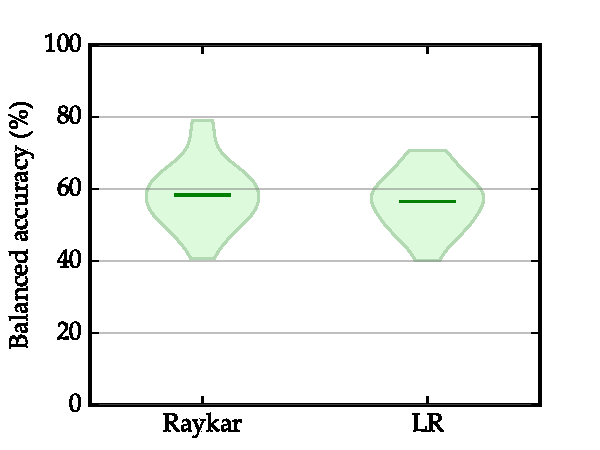
\includegraphics[height=0.3\textheight]
                    {images/experiments/raykar.pdf}
                \caption{Performance of the \citeauthor{raykar10} classifier
                    against logistic regression (LR) on a simulated crowd
                    labelling of the breast cancer dataset \citep{wolberg90}.}
                \label{fig:raykar}
            \end{figure}

            We first used the implementation to perform a simple, simulated
            crowd labelling problem. Five simulated labellers were assigned true
            positive and false positive rates uniformly distributed in the range
            $[0.25, 0.75]$. Each simulated labeller labelled 50\% of the breast
            cancer dataset (Section \ref{sec:breast-dataset}). Random samples of
            75\% of the examples were drawn 20 times and used to train both the
            \citeauthor{raykar10} classifier and a logistic regression
            classifier (using majority vote for the labels). These classifiers
            were tested against the groundtruth of the remaining 25\%. The
            results are plotted in Figure \ref{fig:raykar}. The Raykar
            classifier attained a balanced accuracy of $(58 \pm 8)\%$ and the
            logistic regression classifier attained a balanced accuracy of $(56
            \pm 8)\%$.

            \todo{Conclude.}

        \subsubsection{The Effect of Class Imbalance}

            \begin{figure}
                \centering
                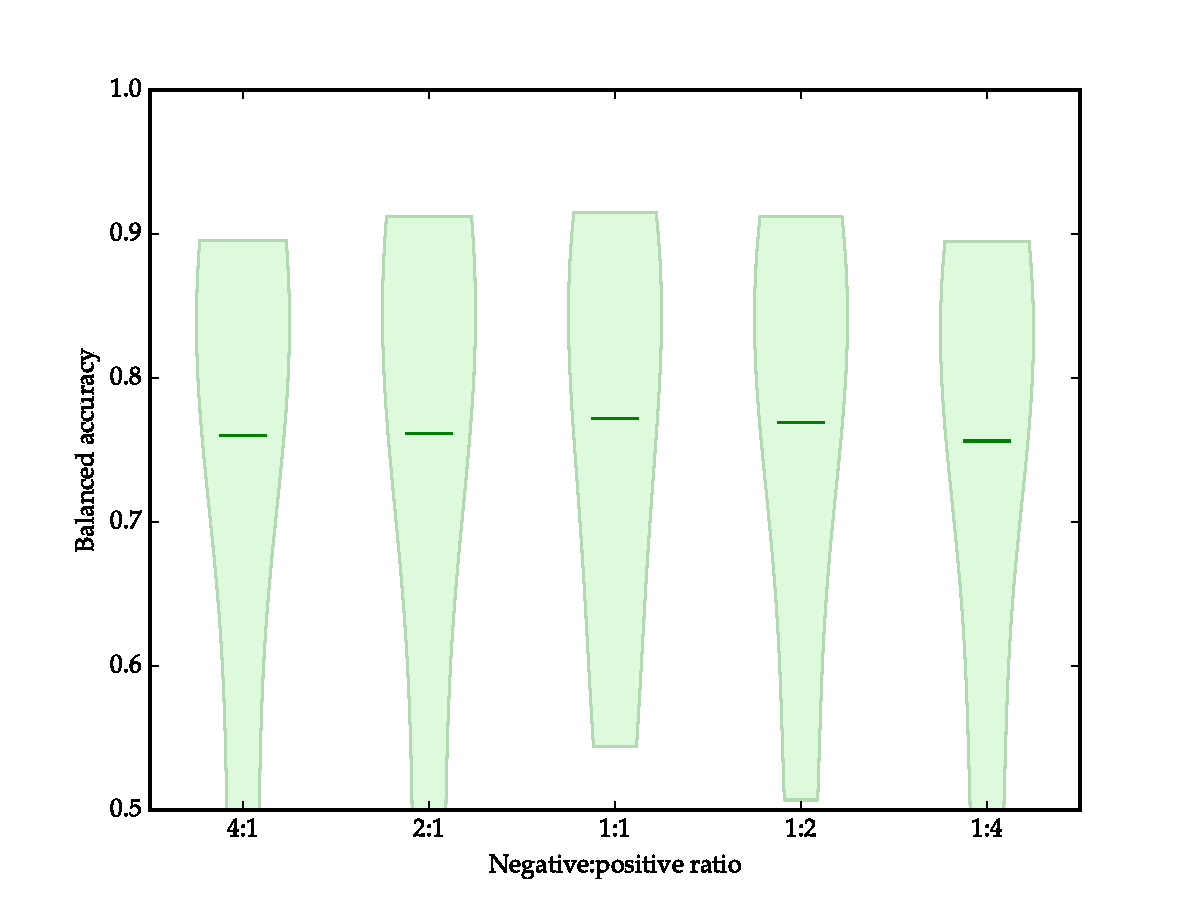
\includegraphics[width=0.8\textwidth]
                    {images/experiments/raykar_class_balance_ba}
                \caption{Performance of the \citeauthor{raykar10} classifier on
                    a simulated labelling problem with different class
                    imbalance.}
                \label{fig:raykar-class-balance-ba}
            \end{figure}

            \begin{figure}
                \centering
                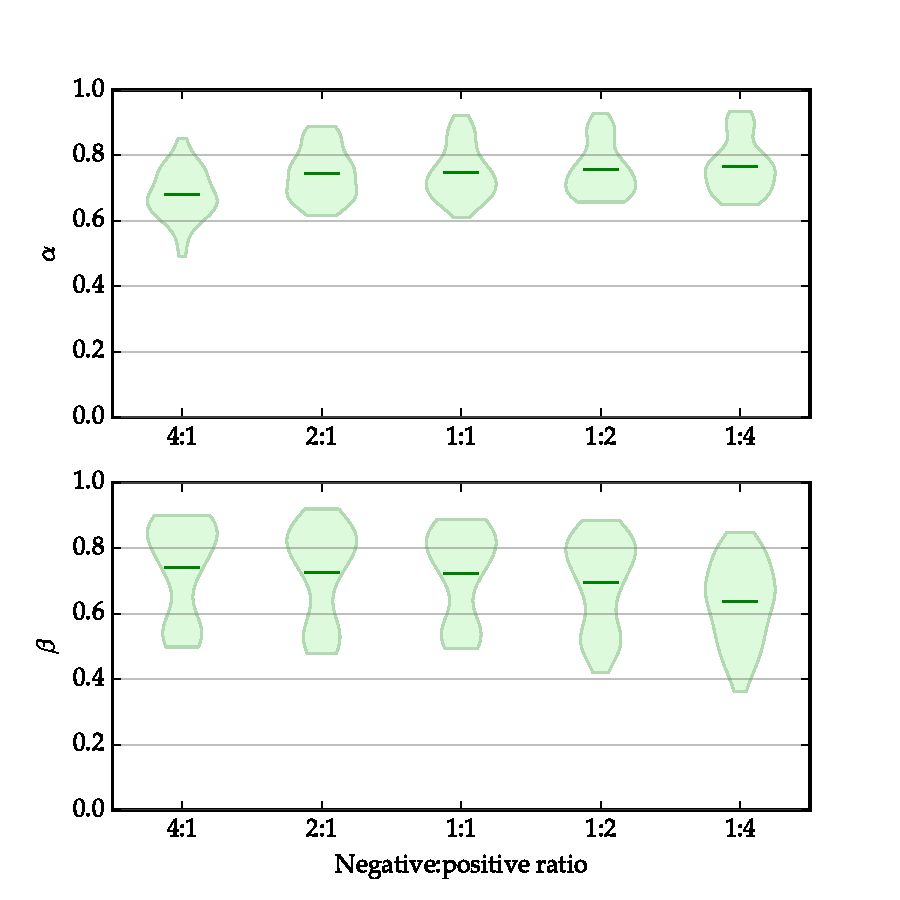
\includegraphics[width=0.8\textwidth]
                    {images/experiments/raykar_class_balance}
                \caption{Output $\alpha$ and $\beta$ values of the
                    \citeauthor{raykar10} classifier on a simulated labelling
                    problem with different class imbalance.}
                \label{fig:raykar-class-balance-ab}
            \end{figure}

            The second experiment tested the effect of class imbalance on the
            resulting balanced accuracy of the classifier, as well as on the
            predicted $\alpha$ and $\beta$ for each labeller. We used
            scikit-learn's \texttt{sklearn.datasets.make\_classification}
            function \citep{scikit-learn} to generate datasets with
            5-dimensional features (of which 3 were informative, and 2 were
            redundant) with a class separation of 1 and 1\% of true labels
            randomly flipped. We generated five datasets, each with 1000
            examples, with different ratios of negative to positive examples.
            The ratios were $4:1$, $2:1$, $1:1$, $1:2$, and $1:4$. We then
            simulated a crowd labelling task as in Section
            \ref{sec:crowd-simulation}, assigning 10 labellers true positive and
            false positive rates uniformly at random in the interval $[0.5,
            0.9]$ and allowing them to ``label'' the examples. The same
            labellers were used across all trials and datasets. We ran the
            \citeauthor{raykar10} algorithm on each dataset and recorded the
            balanced accuracy and output $\alpha$ and $\beta$ values for each
            trial and dataset. We repeated this experiment 5 times. The
            resulting balanced accuracies are plotted against the ratios of
            negative to positive examples in Figure
            \ref{fig:raykar-class-balance-ba}, and the estimated $\alpha$ and
            $\beta$ values are plotted against the ratios in Figure
            \ref{fig:raykar-class-balance-ab}.

            \todo{Conclude.}

            \clearpage

        \subsubsection{The Effect of Label Noise}

            \begin{figure}
                \centering
                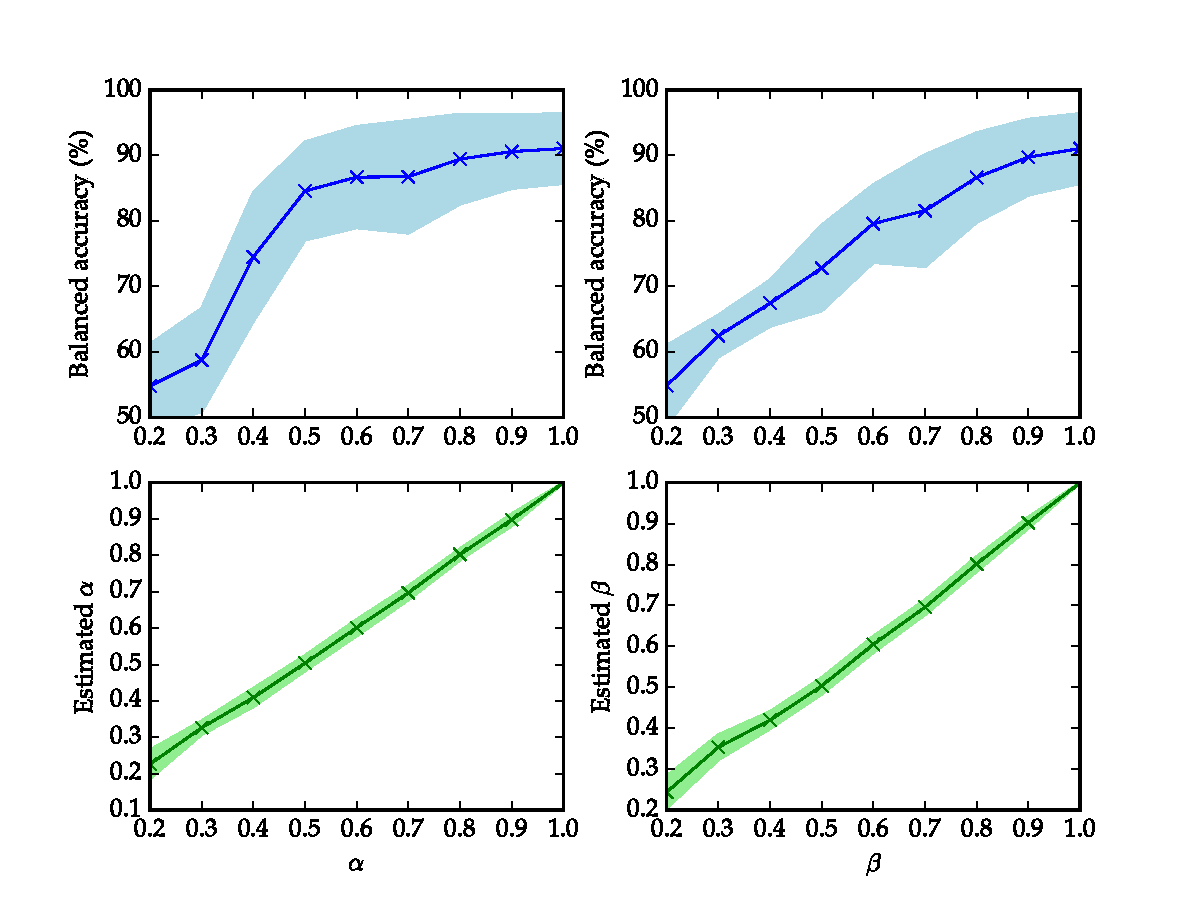
\includegraphics[width=\textwidth]
                    {images/experiments/raykar_noise}
                \caption{Output $\alpha$, $\beta$, and balanced accuracy of the
                    \citeauthor{raykar10} classifier on a simulated labelling
                    problem with different amounts of label noise. ``Estimated
                    $\alpha$'' refers to the value of $\alpha$ output by the
                    algorithm, and $\alpha$ refers to the groundtruth. Filled
                    areas represent the standard deviation of multiple
                    measurements.}
                \label{fig:raykar-noise}
            \end{figure}

            The final experiment was to determine the effect of label noise on
            the performance and output of the algorithm. 10 labellers were
            simulated with $\alpha$ ranging from $0.2$ to $1.0$ and $\beta$
            fixed at $1.0$. A dataset was generated as for the previous
            experiment (but with balanced classes), the labellers were tasked
            with labelling this dataset, and the labels were used to train the
            algorithm. The balanced accuracy and $\alpha$ values were recorded.
            This experiment was repeated $5$ times, and repeated again with
            $\beta$ replacing $\alpha$. The results are shown in Figure
            \ref{fig:raykar-noise}.

            As expected, the balanced accuracy increases as label noise
            decreases. The output $\alpha$ and $\beta$ closely match the true
            values.

    \subsection{Yan et al. Model}
    \label{sec:yan}

        A similar approach is described by \citet{yan10}, again jointly learning
        the groundtruth and labeller models. Unlike \citeauthor{raykar10}, the
        \citeauthor{yan10} labeller model is data-dependent. The accuracy of the
        $t$-th labeller is modelled by a Bernoulli distribution of $\eta_t(\vec
        x)$, parametrised as a logistic regression function $\eta_t(\vec x) =
        \sigma(\vec \omega_t^T \vec x + \gamma_t)$. The labeller model is thus
        \begin{equation*}
            p(y_t \mid \vec x, z, \vec \omega_t, \gamma_t) =
                \eta_t(\vec x)^{1 - |y_t - z|} (1 - \eta_t(\vec x))^{|y_t - z|}.
        \end{equation*}
        For ease of notation, let $\Omega = (\vec \omega_1^T, \dots,
        \vec \omega_T^T)$ and let $\vec \gamma = (\gamma_1, \dots, \gamma_T)$.
        This model can be obtained from the \citeauthor{raykar10} model by
        requiring $\alpha_t = \beta_t = \eta_t(\vec x)$ and allowing these
        parameters be data-dependent.

        As with \citeauthor{raykar10}, the classification model can be any
        classifier and \citeauthor{yan10} choose to use logistic regression
        (Equation \ref{eq:raykar-logreg}). The parameters $\vec \theta =
        \{\Omega, \vec \gamma, \vec w\}$ can be found by maximising the
        likelihood with expectation-maximisation. Under the assumptions that
        examples are independently sampled and that the labellers are
        independent, the likelihood is given by
        \begin{align*}
            p(\mathcal D \mid \vec \theta)
                &= \prod_{i = 1}^N \prod_{t = 1}^T
                    p(y_{t, i} \mid \vec x_i, \vec w, \Omega, \vec \gamma)\\
                &= \prod_{i = 1}^N \prod_{t = 1}^T \sum_{z = 0}^1
                    p(y_t \mid \vec x_i, z, \vec \omega_t, \gamma_t)
                    p(z \mid \vec x_i, \vec w).
        \end{align*}
        The expectation step requires us to compute
        \[
            \mu_i \propto \prod_{t = 1}^{T}
                p(y_{t, i} \mid \vec x_i, z_i = 1, \vec \omega_t, \gamma_t)
                p(z_i = 1 \mid \vec x_i, \vec w).
        \]
        The maximisation step requires us to maximise
        \begin{equation*}
            \sum_{i = 1}^N \sum_{t = 1}^T \sum_{z_i = 0}^1
                p(z_i \mid \vec x_i, \vec w) (
                    \log p(y_{t, i} \mid \vec x_i, z, \vec \omega_t, \gamma_t) +
                    \log p(z \mid \vec x_i, \vec w))
        \end{equation*}
        with respect to $\vec w, \Omega,$ and $\vec \gamma$, where $p(z_i \mid
        \vec x_i, \vec w)$ is fixed to use the previous value of $\vec w$.

        As part of this thesis, we have produced an open source implementation
        of this algorithm, described in Section \ref{sec:crowdastro-yan}. After
        the algorithm was implemented, we found it to be considerably slower
        than the \citeauthor{raykar10} algorithm, so we do not use it later in
        this thesis. Its main purpose here is to show that the expectation-
        maximisation approach can be extended by choice of labeller model.

        \begin{figure}
            \centering
            \begin{subfigure}{\textwidth}
                \centering
                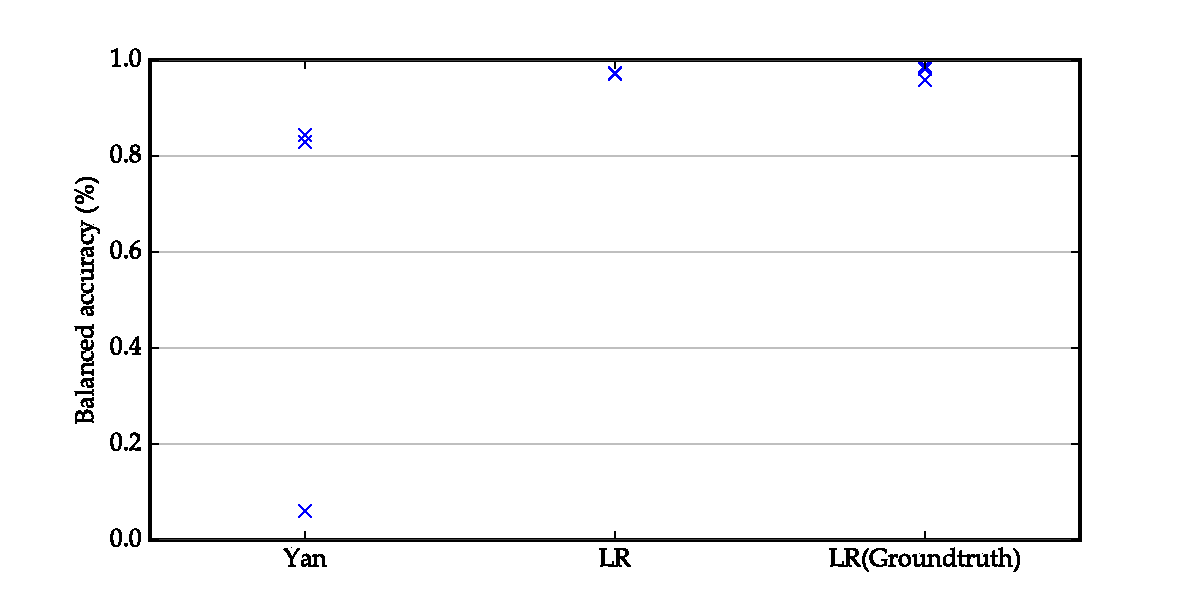
\includegraphics[width=0.9\textwidth]
                    {images/experiments/yan_25pc_noise.pdf}
                \caption{$\upsilon = 75\%$}
                \label{fig:yan-experiment-low-noise}
            \end{subfigure}
            \begin{subfigure}{\textwidth}
                \centering
                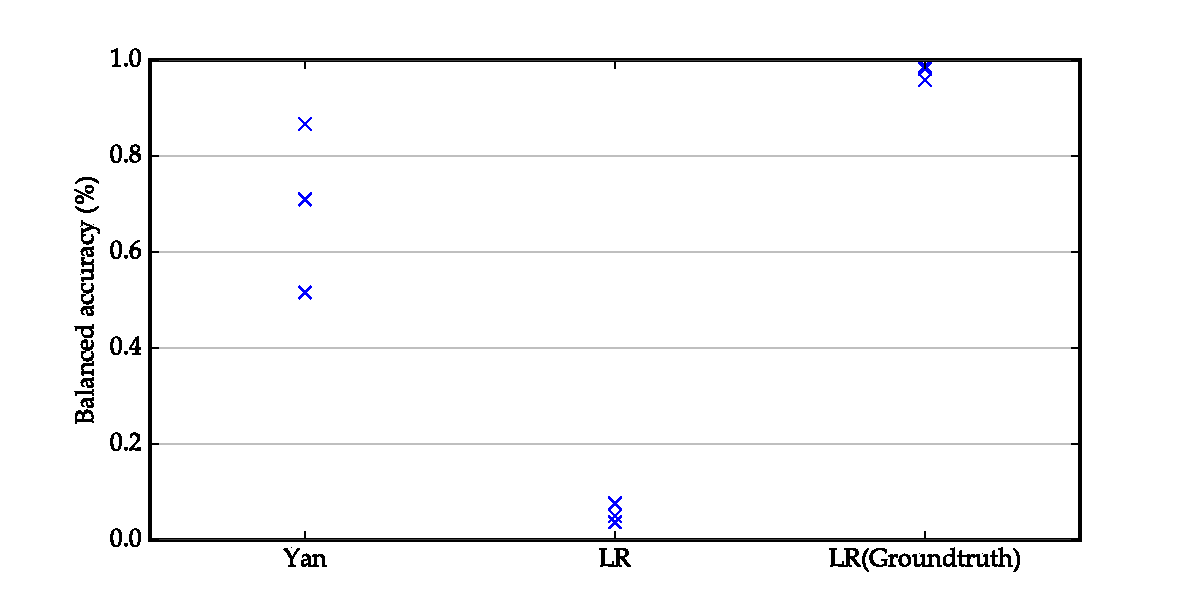
\includegraphics[width=0.9\textwidth]
                    {images/experiments/yan_75pc_noise.pdf}
                \caption{$\upsilon = 25\%$}
                \label{fig:yan-experiment-high-noise}
            \end{subfigure}
            \caption{\citeauthor{yan10} algorithm compared with logistic
                regression trained on the majority vote (LR) and logistic
                regression trained on the groundtruth (LR(Groundtruth)).
                Labellers have an accuracy of $\upsilon$ when not in
                their cluster of expertise.}
        \end{figure}

        The \citeauthor{yan10} algorithm is good for modelling labellers with
        highly feature-dependent noise. To test the algorithm, we employed it on
        the breast cancer Wisconsin dataset (Section \ref{sec:breast-dataset}),
        but using a different simulation of labellers to that used for the
        \citeauthor{raykar10} tests of Section \ref{sec:raykar}. While the
        method for generating simulated crowd labels was similar, the labeller
        model differed to show the ability of the \citeauthor{yan10} model to
        handle feature-dependent noise. Instead of using two values $\alpha$ and
        $\beta$ to describe each labeller, we clustered the data and assigned
        each labeller one cluster The labeller had $100\%$ accuracy for that
        cluster, and a fixed lower accuracy $\upsilon$ for all other clusters,
        giving each labeller a ``cluster of expertise''.. We tested with low
        noise ($\upsilon = 0.75$) and high noise ($\upsilon = 0.25$). The
        results are compared with logistic regression trained on the majority
        vote and logistic regression trained on the groundtruth in Figure
        \ref{fig:yan-experiment-low-noise} and Figure
        \ref{fig:yan-experiment-high-noise} for low and high noise,
        respectively.

        From these plots, we can tell that with low noise, logistic regression
        is able to learn a high quality model from the majority vote, while the
        \citeauthor{yan10} model performs more poorly. While it is possible for
        the \citeauthor{yan10} model to reduce to logistic regression, this is
        evidently not guaranteed in practice. This may be due to the difficulty
        of the expectation-maximisation problem, which is never guaranteed to
        converge on a global maximum in general. When noise is high, however,
        the \citeauthor{yan10} algorithm considerably outperforms logistic
        regression, indicating that in situations with high, feature-dependent
        noise, the \citeauthor{yan10} algorithm may be a good choice of
        classification algorithm. However, this choice of labeller model may not
        be ideal with large numbers of labellers. There are $ND$ parameters, so
        the expectation-maximisation algorithm may converge considerably slower
        and the number of local minima may quickly increase with increasing
        numbers of labellers.
